\chapter{OVERVIEW ABOUT PROJECT}

\renewcommand{\headrulewidth}{0.5pt}
\renewcommand{\footrulewidth}{0.5pt}
\thispagestyle{plain}
\pagestyle{fancy}
\fancyhf{}
\fancyhead[L]{\textbf{CHAPTER 1}}
\fancyhead[R]{\textbf{DANGEGOUS WEAPONS DETECTION USING YOLOv9}}
\raggedright
\fancyfoot[L]{From: Nguyen Van Anh Tuan}
\fancyfoot[R]{Page \thepage}

\justifying

\section{Introduction}
    In today's world, terrorism remains a pervasive and evolving threat, posing significant challenges to global security and stability. The methods and tactics employed by terrorists have become increasingly sophisticated, necessitating advanced technological solutions to effectively counteract these dangers. One such critical area is the detection of dangerous weapons, which requires innovative approaches to ensure the safety of populations and the integrity of public spaces. \\ 
    \vspace{3mm}
    This report focuses on the pressing issue of contemporary terrorism and the urgent need for state-of-the-art information tools to detect and neutralize threats. Specifically, we will explore the application of \textbf{YOLOv9(You Only Look Once, version 9)}  technology in identifying dangerous weapons. \textbf{YOLOv9} represents the latest advancement in real-time object detection, offering unparalleled accuracy and speed in recognizing potential threats.
    \vspace{3mm}
    By integrating \textbf{YOLOv9} technology into security frameworks, authorities can significantly enhance their ability to detect concealed weapons and other hazardous materials. This capability is crucial in preempting terrorist activities and mitigating the risks posed by armed attacks. Through a detailed examination of \textbf{YOLOv9} functionalities, performance metrics, and real-world applications, this report aims to underscore its potential in transforming counter-terrorism strategies.
    \vspace{3mm}
    In the following sections, we will delve into the mechanics of \textbf{YOLOv9}, its advantages over previous versions, and its practical implementation in various security scenarios. By leveraging cutting-edge technology, we can better equip our security forces to anticipate and respond to the ever-changing landscape of terrorist threats, ultimately safeguarding our societies against the scourge of terrorism.

\section{Why YOLOv9?}
    Choosing YOLOv9 over previous versions of YOLO (such as YOLOv8 or earlier) can offer several advantages. Here are some compelling reasons:
    \begin{itemize}
        \item \textbf{Improved Accuracy:} YOLOv9 typically comes with enhanced algorithms and architectures that increase the accuracy of object detection. This includes better localization of objects and more precise classification.
        \item \textbf{Higher Speed:} Despite the improved accuracy, YOLOv9 is optimized for speed, maintaining or even increasing the inference speed compared to its predecessors. This makes it suitable for real-time applications.
        \item \textbf{Advanced Features:} YOLOv9 may incorporate new features like better handling of small objects, improved multi-scale detection, and more robust handling of overlapping objects.
        \item \textbf{Better Generalization:} Enhanced training techniques and data augmentation strategies in YOLOv9 can lead to better generalization across different datasets and environments, reducing overfitting.
        \item \textbf{Reduced Computational Requirements:} YOLOv9 might offer improved efficiency, requiring less computational power or memory while achieving superior performance, making it accessible for deployment on edge devices or less powerful hardware.
        \item \textbf{Enhanced Backbone and Head Networks:} The architecture of YOLOv9 often includes more advanced backbone networks (like CSPNet, EfficientNet) and head networks that contribute to better feature extraction and object detection capabilities.
        \item \textbf{Improved Training Mechanisms:} YOLOv9 could come with advanced training methodologies such as self-supervised learning, knowledge distillation, or semi-supervised learning, improving model performance with less labeled data.
        \item \textbf{Compatibility and Integration:} YOLOv9 might offer better integration with modern frameworks, libraries, and deployment tools, facilitating easier implementation in diverse projects and workflows.
        \item \textbf{State-of-the-Art Techniques:} YOLOv9 is designed to incorporate the latest research in computer vision and deep learning, ensuring that users have access to state-of-the-art techniques and methodologies.
    \end{itemize}
    Choosing the latest version like YOLOv9 ensures that you are leveraging the most recent advancements in object detection technology, leading to improved performance and capabilities in your projects.

\section{Target and The Limits of Project}
    \subsection{Target of Project}
    This project is the first step to learn about the application of processed images in reality, at the same time is also 
    a step to deploy the learned knowledge. Through research and serious work to practice manners, as well as perfecting 
    methods, researching thinking and solving a problem. With the objectives of the project is:
    \begin{itemize}
        \item Developing an Accurate Detection Model
        \item Real-time Detection Capabilities
        \item Learn about image processing
        \item Learn about YOLO, Python
        \item Install library for YOLO, Ikomia
        \item Real-time Detection Capabilities
        \item Comprehensive Documentation and Training
        \item Write program
        \item Experimental model
        \item Developing an Accurate Detection Model
    \end{itemize}
    \subsection{Limitation of Project}
    \begin{itemize}
        \item The limitation of this project is the inability to detect weapons when processing through colorless video
        \item Cannot detect when the distance of the object is too far from the camera
        \item There is no device powerful enough to be able to train on a huge amount of data
        \item Limitation of Google Colab environment when using too much GPU
    \end{itemize}

\section{Workflow of Project}
    \begin{figure}[H]
        \centering
        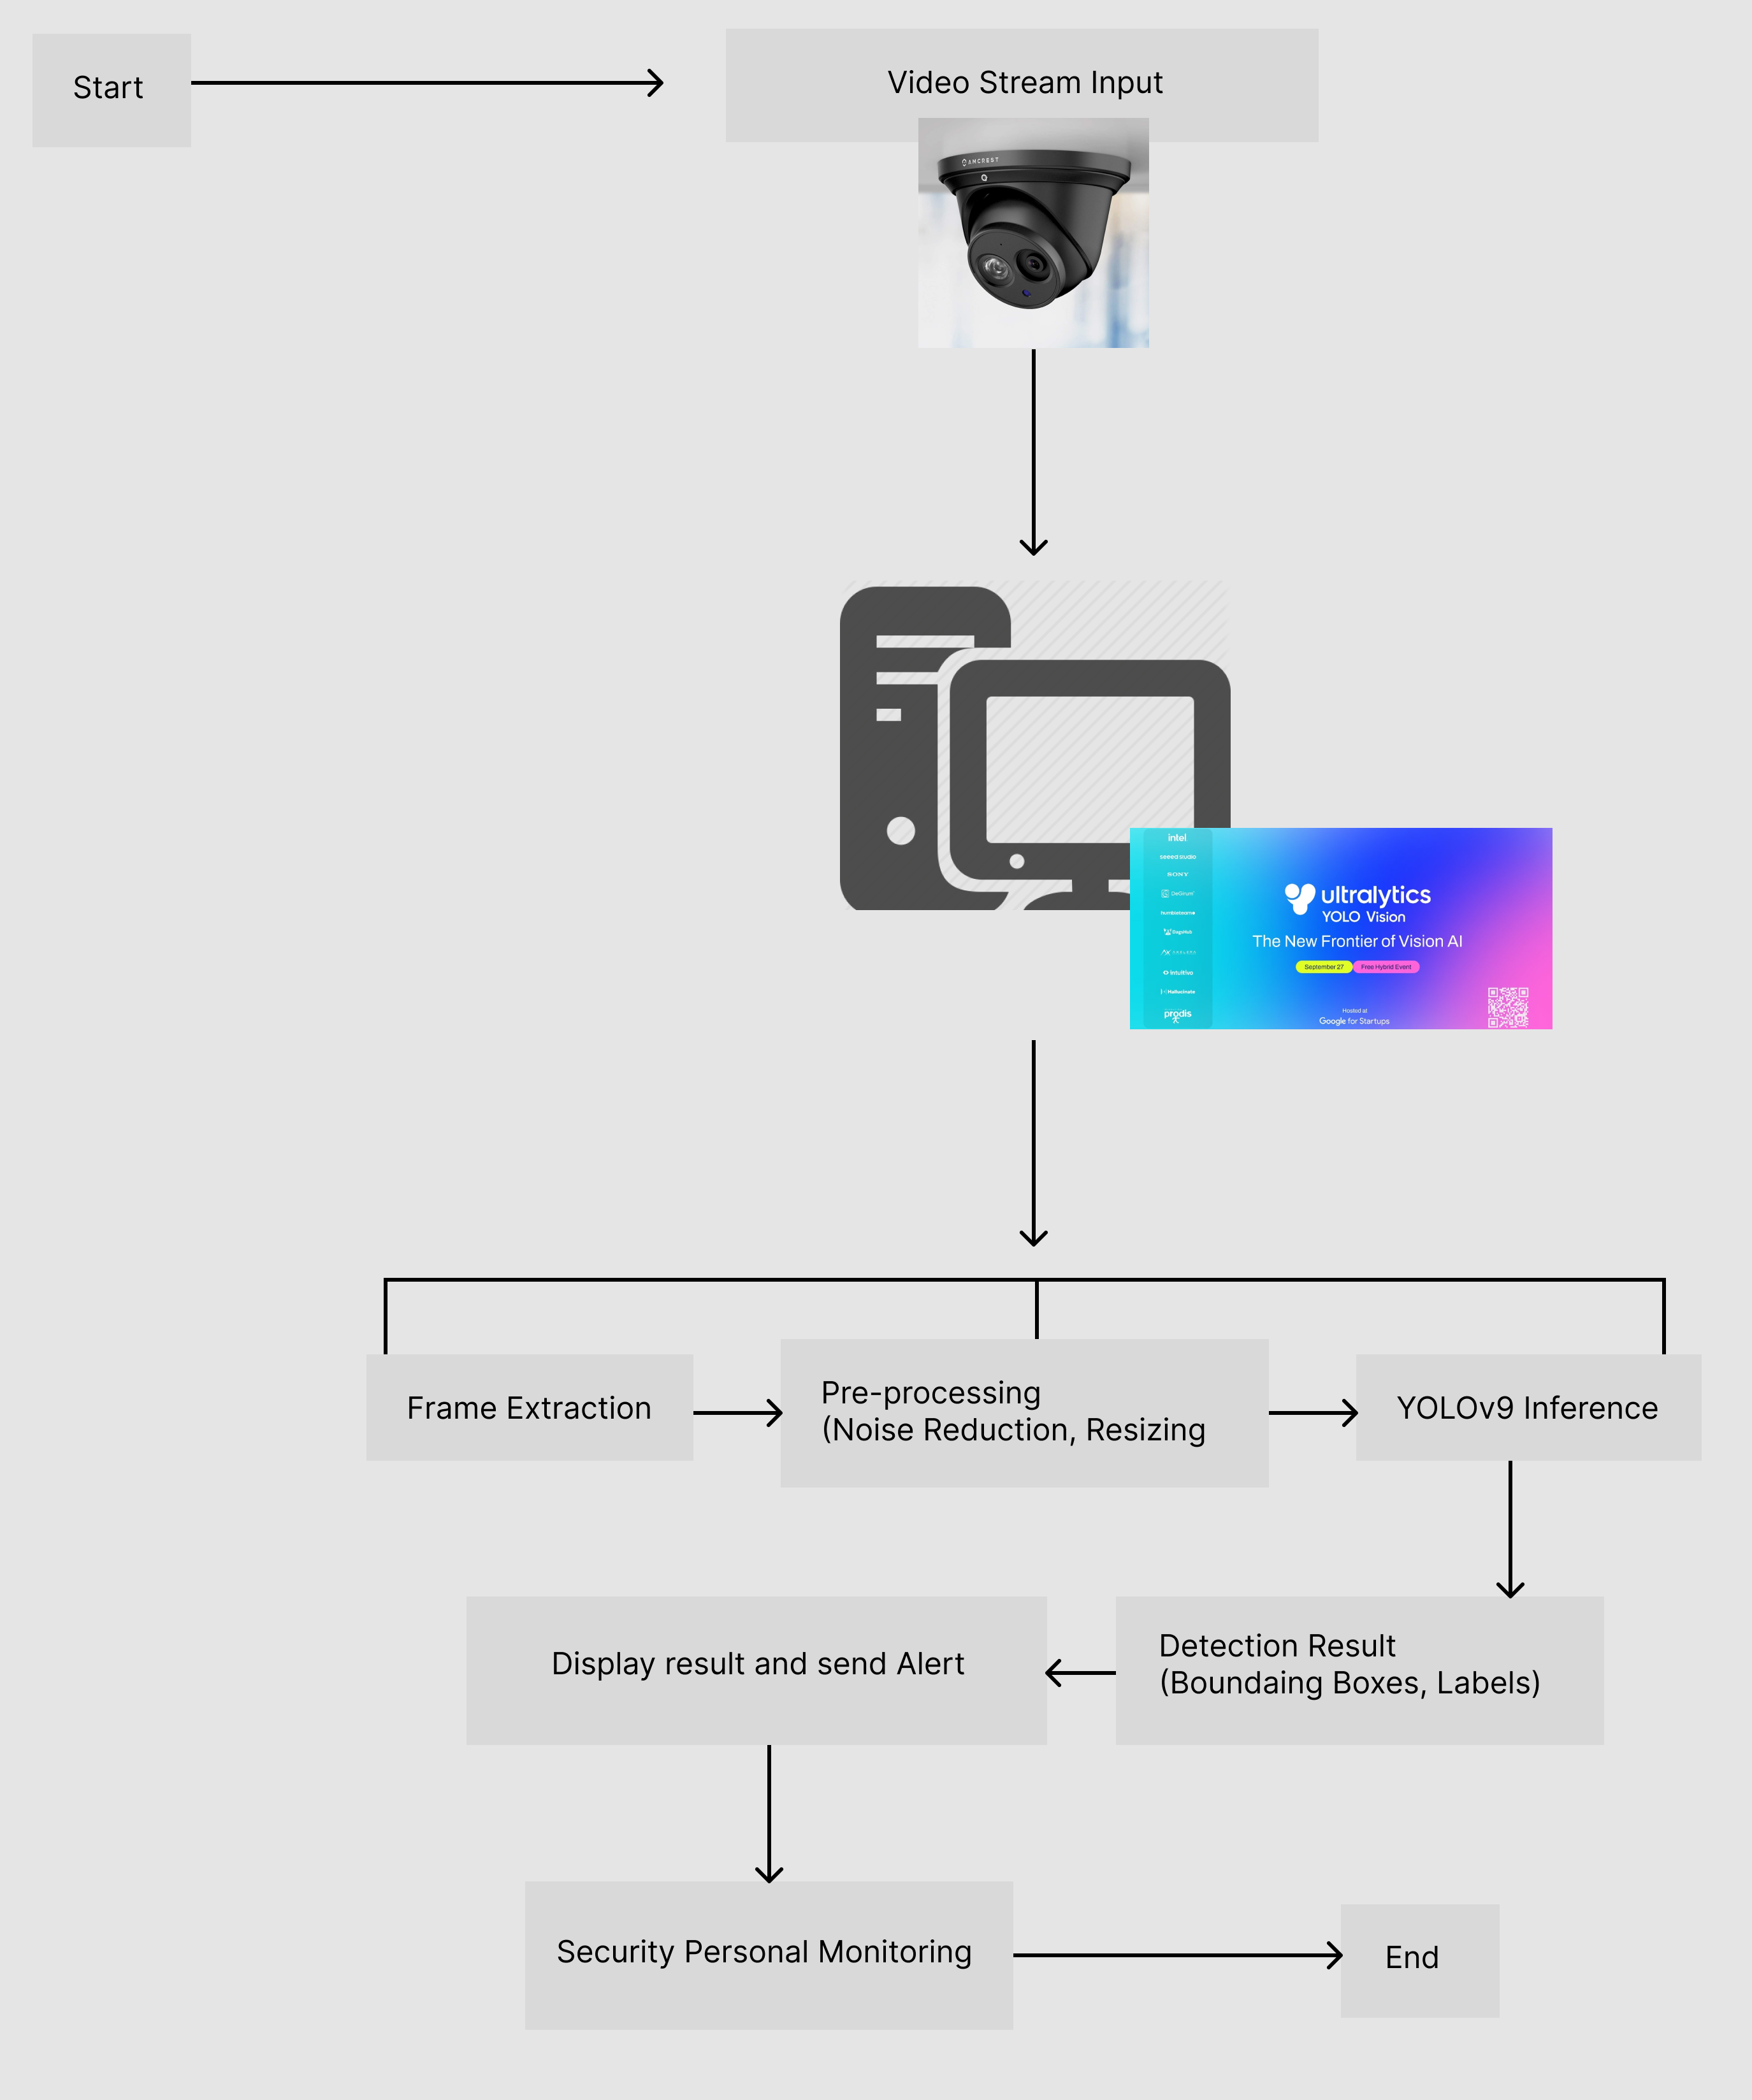
\includegraphics[width=0.8\linewidth]{img/Diagram.png}
        \caption{Block Diagram of Project}
        \label{fig:diagram}
    \end{figure}